\chapter{Signal fit}
\label{sec:Signalfit}
This chapter describes the way how the signal yield \NLc of the signal channel \LbToDpmunuX is derived.
As already explained in section \ref{sec:Strategy} the aim is to perform a twodimensional fit in the \Dz\proton mass and \logIP distribution.
The \logIP distribution enables the fit to distinguish (nonresonant) signal from random proton background.
This information is used in the \MDp dimension to separate the different components and to learn more about the \MDp spectrum.
From other experiments it is expected that there should appear the two resonances \decay{\LcResI}{\Dz\proton} and \decay{\LcResII}{\Dz\proton} \cite{BaBar_D0p}.
Before the fit can be performed, a proper parametrization of the fit components has to be found. 
This will be described in the following section.

\section{Getting the fit parametrization}
Different approaches are used to model the components of the fit. 
The discussion will be separated in the weo fit dimensions starting with the \logIP shape.

\subsection{\logIP shape}
For both, \logIP signal and background components, simulations are used. 
The signal part can be described by a sum of two Bifurcated Gaussians.
A Bifurcated is like a Gaussian, but with two different widths for the left and the right part from the maximum and thus providingan ``asymmetric Gaussian".
If $\mathcal{G}(m|m_0,\sigma)$ denotes a usual Gaussian with mean $m_0$ and width $\sigma$, a Bifurcated Gaussian can be written as\footnote{All fitfunctions in the following are given without normalisation factors. That's why there always appears a $\propto$ sign instead of an equal sign.}
\begin{align}
    \text{BfG}(m|m_0, \sigma_{\text{L}}, \sigma_{\text{R}}) \propto 
    \begin{cases}
        \mathcal{G}(m|m_0,\sigma_{\text{L}}) & \text{for } m < m_0 \\   
        \mathcal{G}(m|m_0,\sigma_{\text{R}}) & \text{for } m > m_0 \\   
    \end{cases},
\end{align}
and the sum of two is in the following called a double Bifurcated Gaussian DBfG
\begin{align}
    \text{DBfG}(m|m_0,\vec{\sigmaL{}}, \vec{\sigmaR{}}, f_{\BfG_1}) \propto \\
    f_{\BfG_1} \BfG(m|m_0,\sigmaL{1}, \sigmaR{1}) + \left(1 - f_{\BfG_1} \right) \BfG(m|m_0,\sigmaL{2}, \sigmaR{2}),
\end{align}
where $f_{\BfG_1}$ denotes the fraction of the first \BfG and the two \BfG share a common mean $m_0$. The fitresult on the signal simulation can be seen in figure \ref{fig:fit_logIP_signal}.
\begin{figure}[hptb]
    \centering
	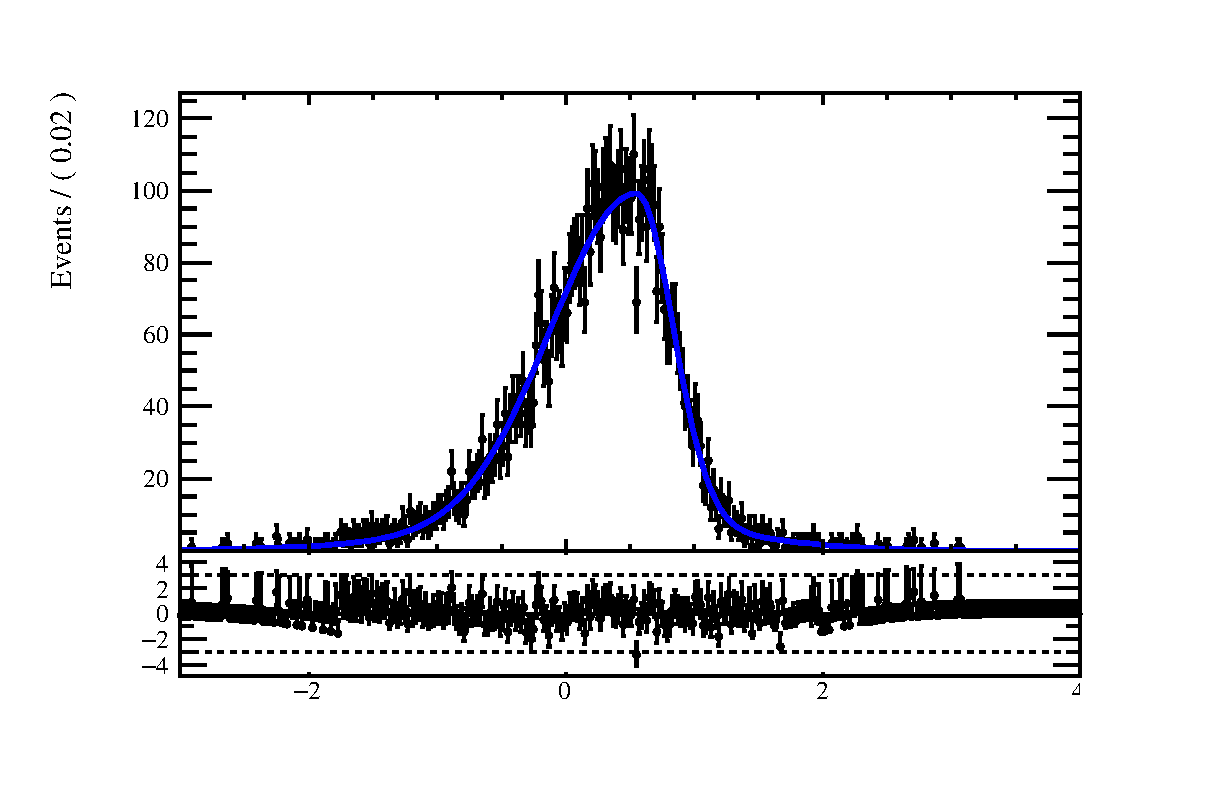
\includegraphics[width=0.49\textwidth]{LbToD0p/fits/MC_D0p_SIG/logIP_RS/fit_DBfG}
	\caption{Fit to the \logIP distribution of the signal simulation. As parametrization a double Bifurcated Gaussian has been chosen.}
    \label{fig:fit_logIP_signal}
\end{figure}

Concerning the background shape only a simulation with very few statistics is available.
To get a better idea of the background \logIP shape right sign and wrong sign events of this sample have been added.
Since in this case they are both backgrounds with respect to the \logIP signal it is assumed that their shapes are similar as figure \ref{fig:plot_logIP_MC_BKG} confirms. 
As fitfunction a single CrystalBall function is chosen. 
This function was first used by the CrystalBall collaboration to account for radiative losses in \jpsi or \psitwos decays \cite{CrystalBall}. It is defined as 
\begin{align}
    &\CB(m|m_0, \sigma, \alpha, n) \propto
    \begin{cases}
        \exp \left(-\frac{(m-m_0)^2}{2\sigma^2}\right)     & \text{for } \frac{m-m_0}{\sigma} > -\alpha \\
        A \cdot \left(B - \frac{m-m_0}{\sigma}\right)^{-n} & \text{for } \frac{m-m_0}{\sigma} \leq -\alpha
    \end{cases}, \\
    &\text{where} \\
    &A = \left(\frac{n}{|\alpha|}\right)^n \exp\left(-\frac{|\alpha|^2}{2}\right), \\
    &B = \frac{n}{|\alpha|} - |\alpha|.
\end{align}
The CrystalBall function is hence a Gaussian with a power law tail. 
The result of the fit to the background simulation can be seen in figure \ref{fig:fit_logIP_MC_BKG}.
\begin{figure}[hptb]
    \centering
	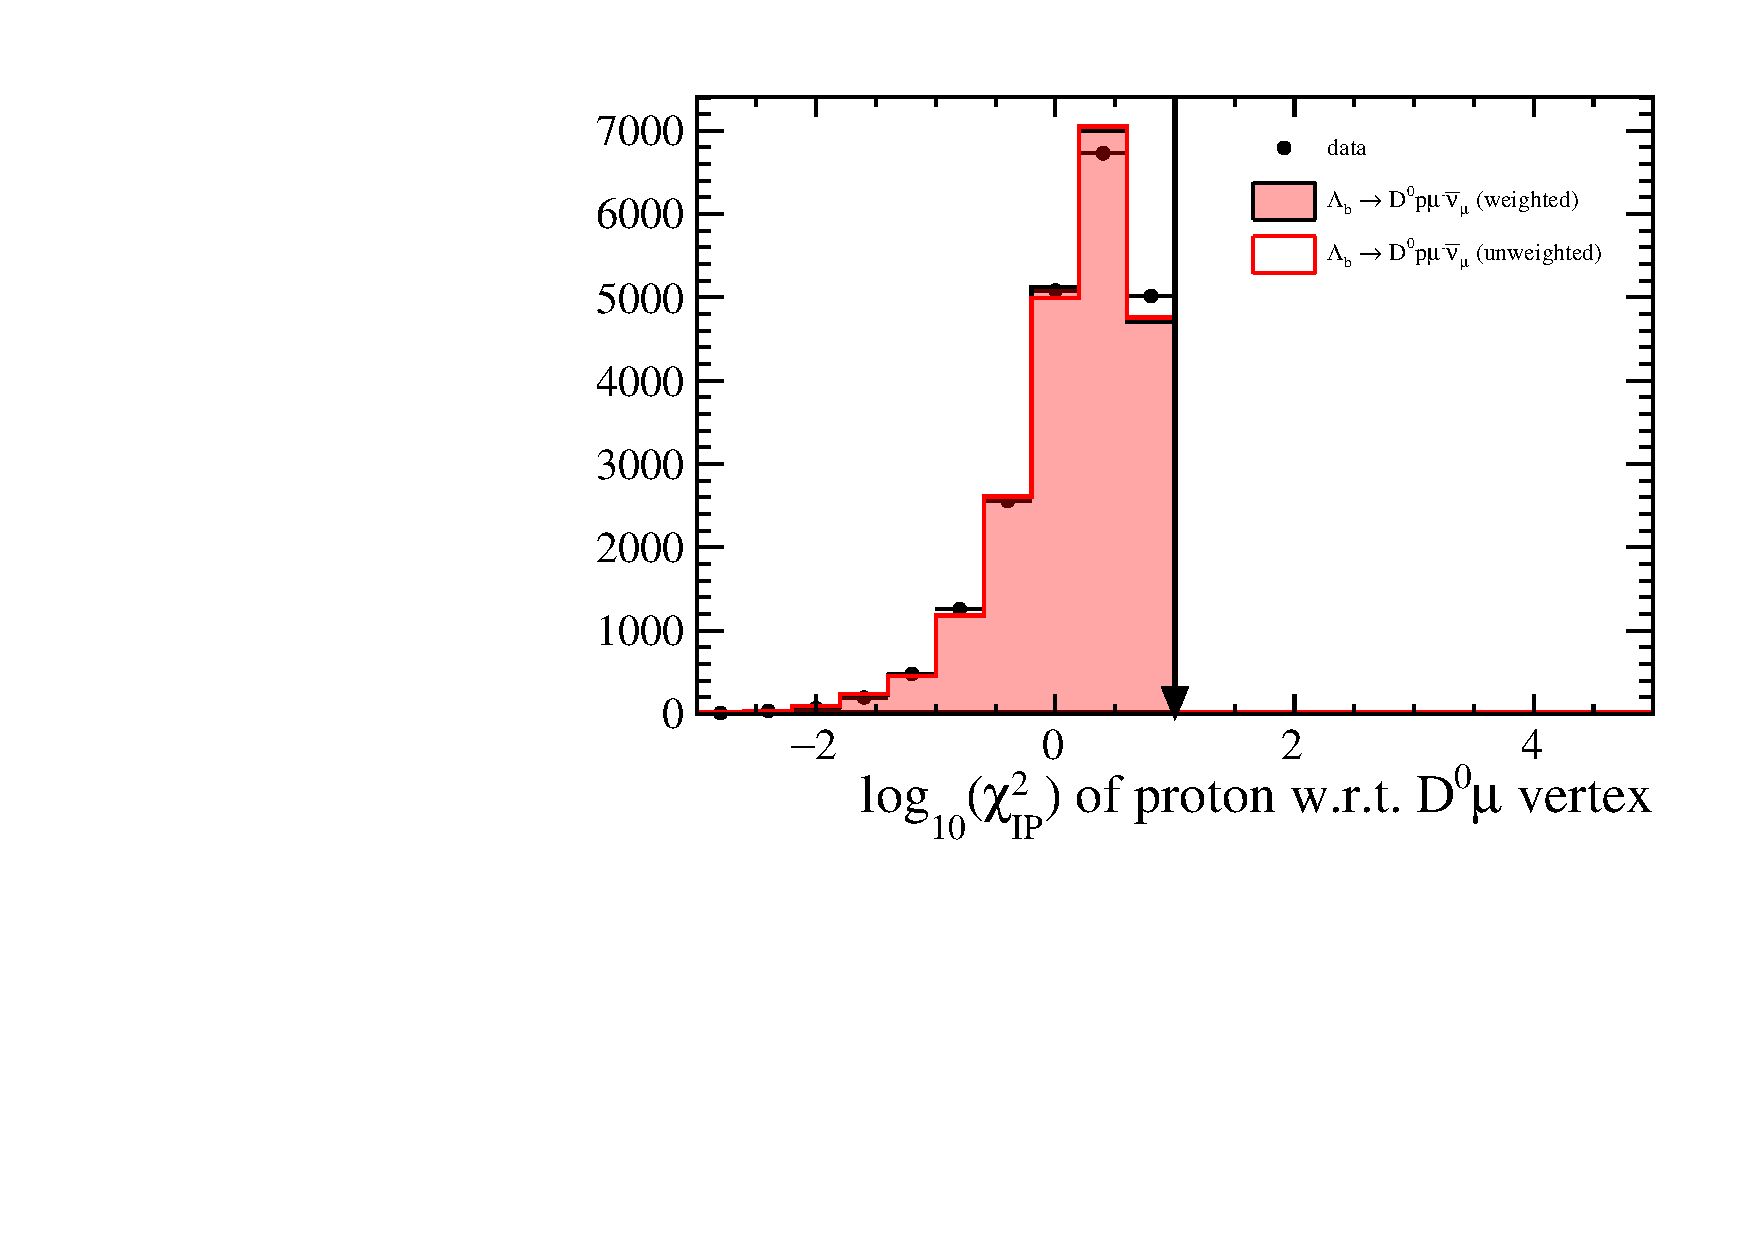
\includegraphics[width=0.49\textwidth]{LbToD0p/plots/MC_B2D0munu_BKG/logIP}
	\caption{Comparison of RS and WS events in the background MC. Both, RS and WS shapes are very similar and can thus be added to increase statistics.}
    \label{fig:plot_logIP_MC_BKG}
\end{figure}
\begin{figure}[hptb]
    \centering
	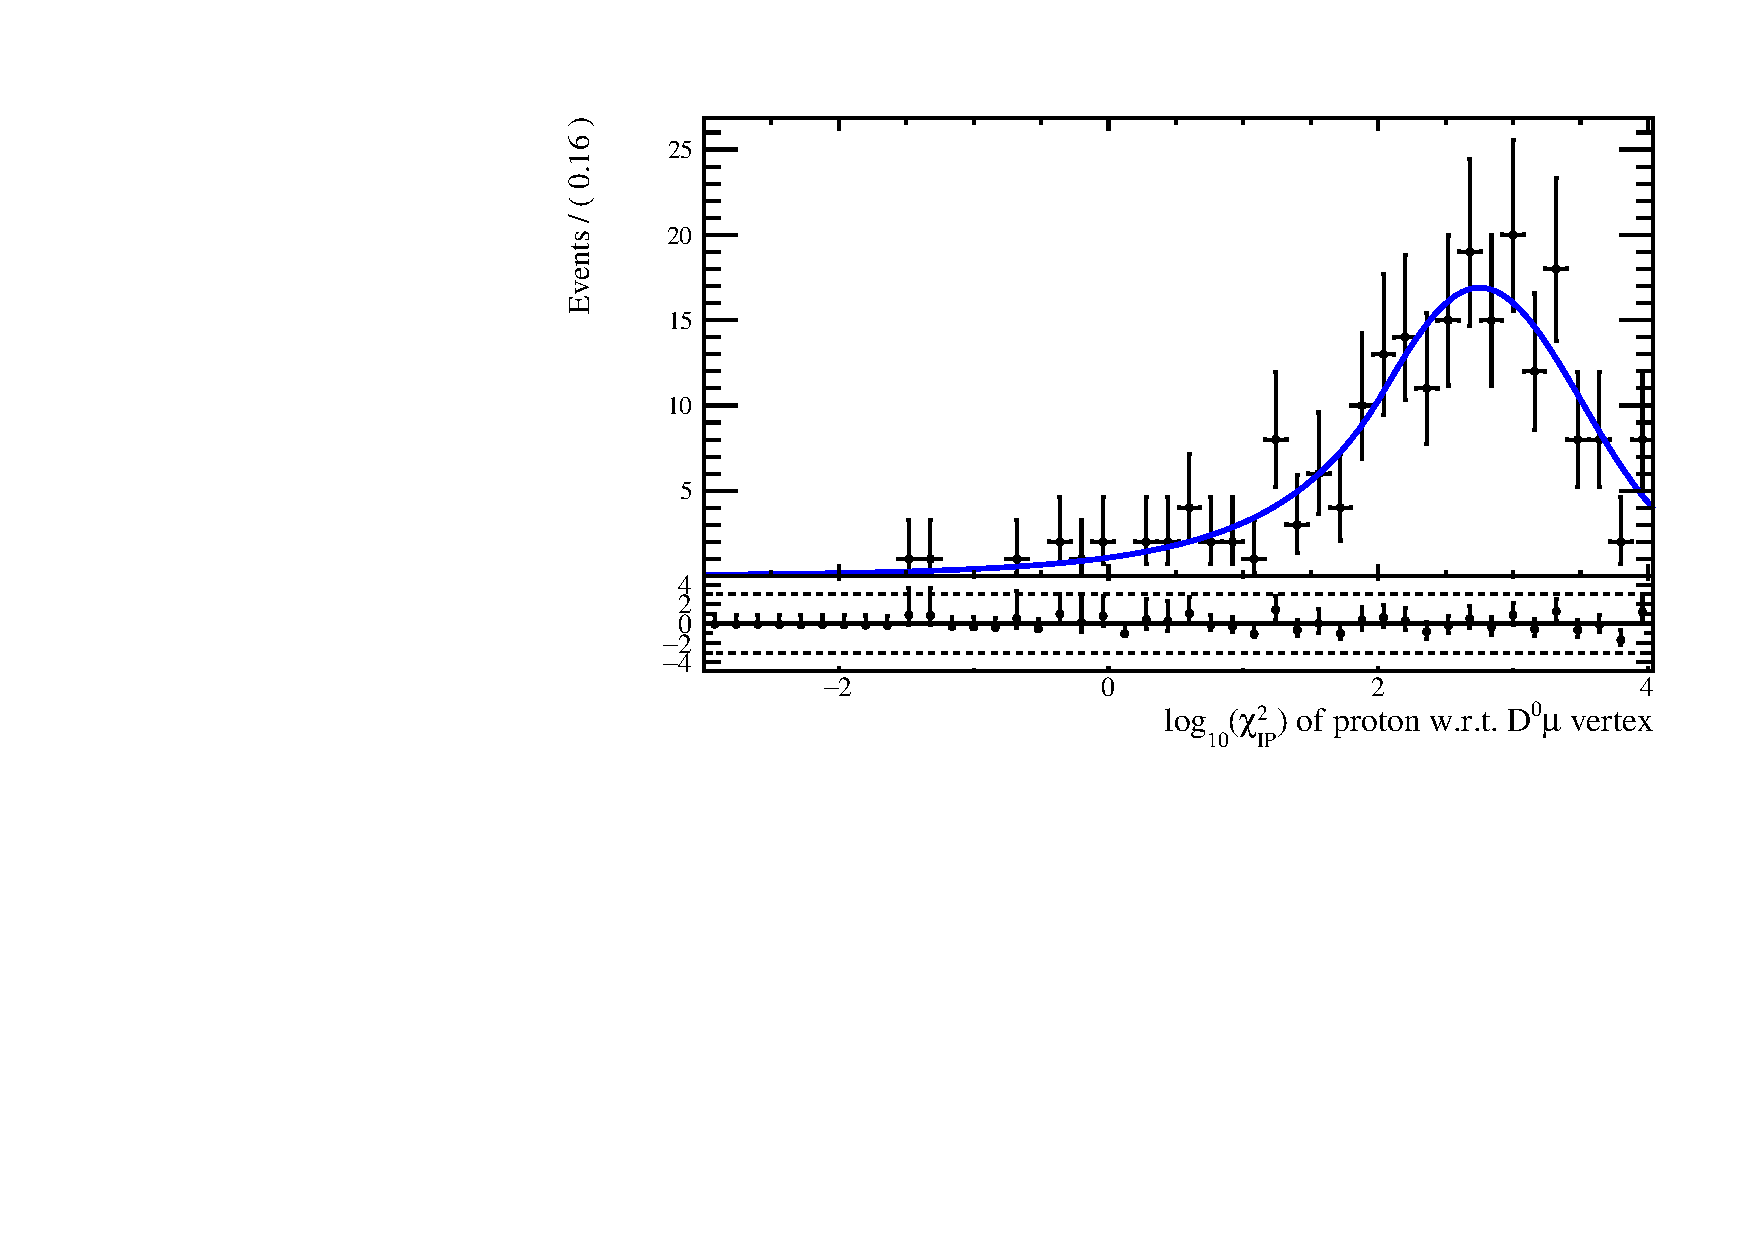
\includegraphics[width=0.49\textwidth]{LbToD0p/fits/MC_B2D0munu_BKG/logIP_RS/fit_CB}
	\caption{Fit to the (RS and WS added) \logIP shape of the background simulation.}
    \label{fig:fit_logIP_MC_BKG}
\end{figure}

\subsection{Control of \logIP parametrization}
\label{sec:ControlLogIP}
As a control of the chosen parametrization of \logIP for signal and background, a onedimensional fit on data is performed. 
This fit is later also used for systematic studies, since it is already able to distinguish between signal and background yields.
The fitresult with the models mentioned above can be seen in figure \ref{fig:fit_logIP_RS} and the corresponding yields and parameter values in table \ref{tab:logIP_RS}.
The chosen model nicely describes the data.
\begin{figure}[hptb]
    \centering
	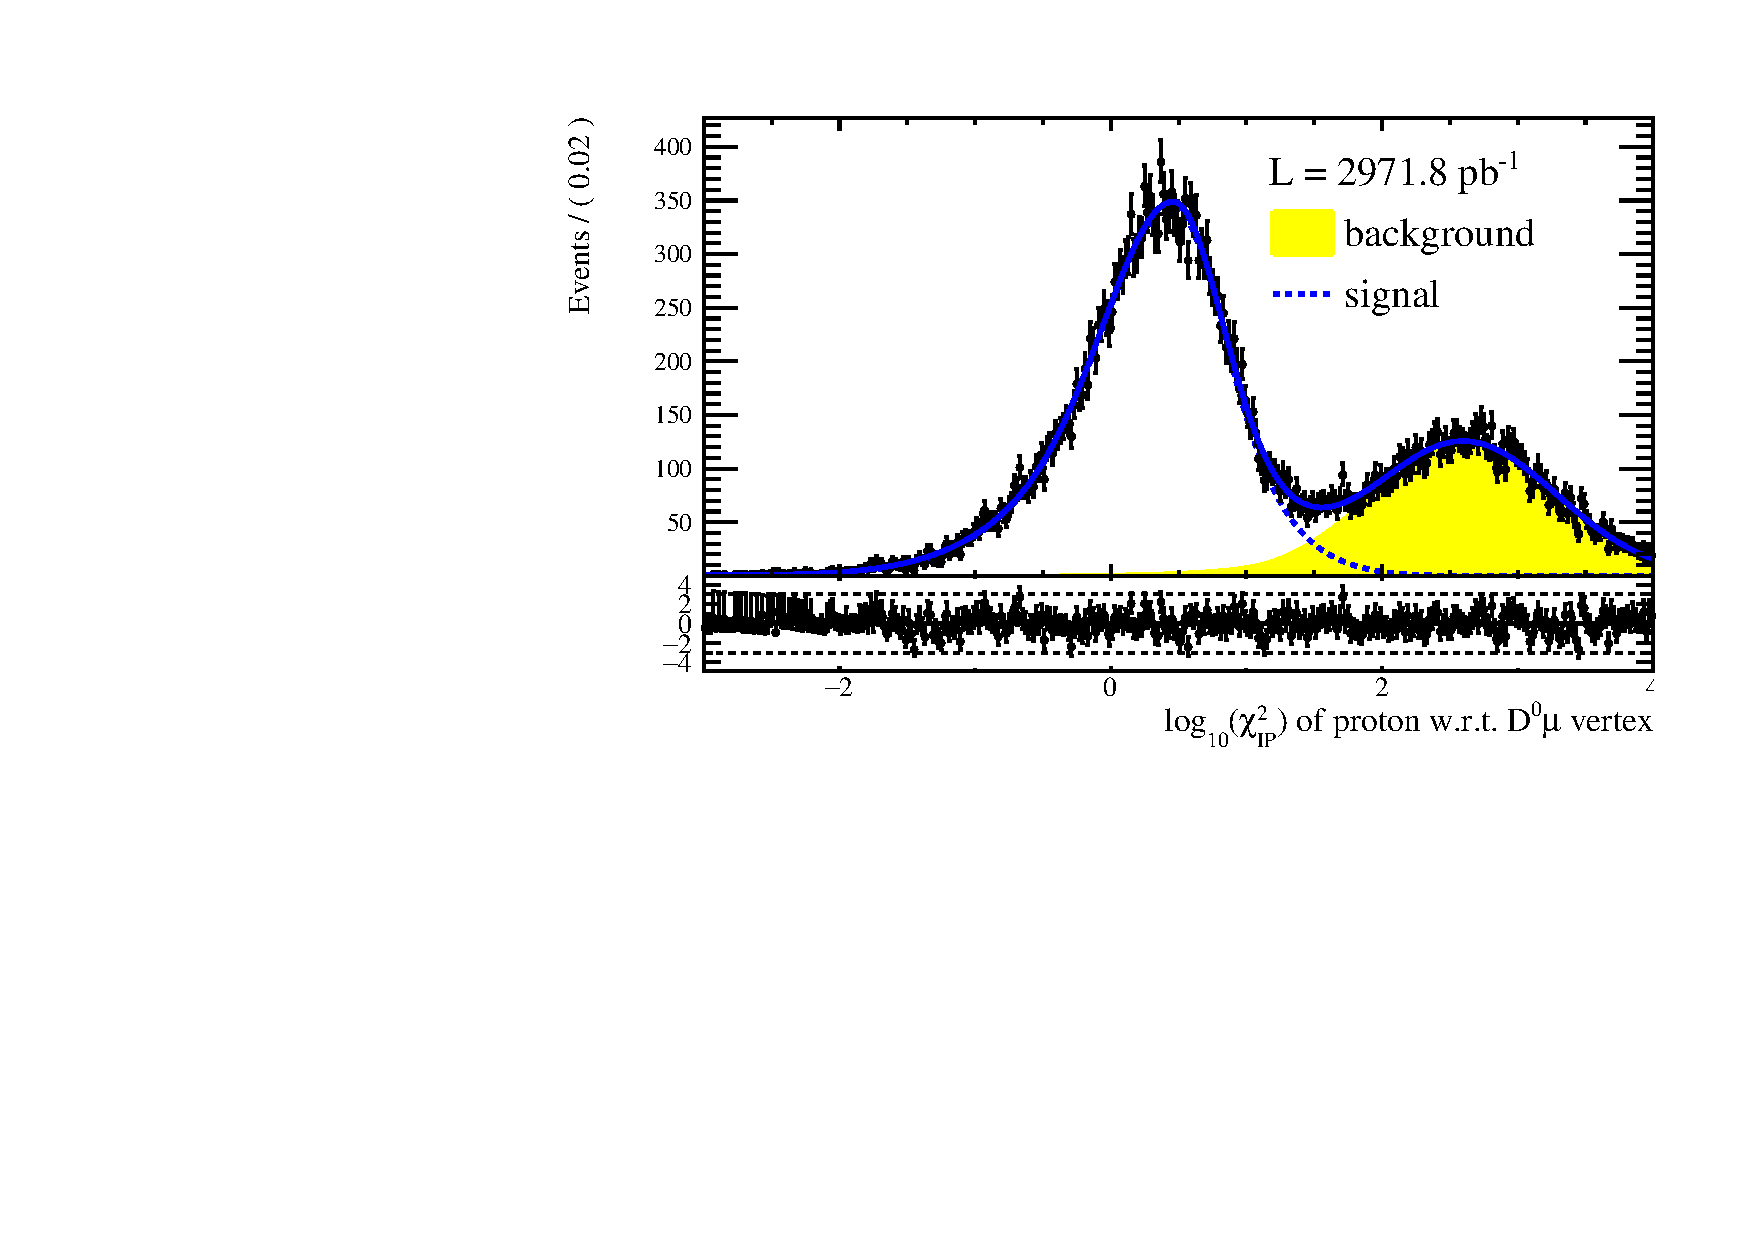
\includegraphics[width=\textwidth]{LbToD0p/fits/data/logIP_RS/fit_DBfG_CB}
	\caption{Fit to the \logIP distribution of the data sample.}
    \label{fig:fit_logIP_RS}
\end{figure}
 
\begin{table}[h]
    \centering
    \caption{Results of the onedimensional \logIP fit on data.}
    \label{tab:logIP_RS}
    $\begin{array}{lr@{\pm}l}
    \hline
    \text{Variable} & \multicolumn{2}{c}{\text{Value}} \\
    \hline
        \multicolumn{3}{l}{\text{\textbf{Yields}}} \\
\text{signal yield}&(2.325 & 0.028) \cdot 10^{4}\\
\text{background yield}&(1.086 & 0.026) \cdot 10^{4}\\
\multicolumn{3}{l}{\text{\textbf{Signal (\DBfG)}}} \\
\text{mean}&(4.59 & 0.26) \cdot 10^{-1}\\
\text{left width 1}&(8.72 & 0.56) \cdot 10^{-1}\\
\text{right width 1}&(5.74 & 0.44) \cdot 10^{-1}\\
\text{left width 2}&(4.72 & 0.55) \cdot 10^{-1}\\
\text{right width 2}&(3.37 & 0.23) \cdot 10^{-1}\\
\text{fraction BfG 1}&(5.61 & 0.89) \cdot 10^{-1}\\
\multicolumn{3}{l}{\text{\textbf{Background (\CB)}}} \\
\text{CB mean}&(2.6 & 0.017) \cdot 10^{0}\\
\text{CB $\sigma$}&(6.85 & 0.14) \cdot 10^{-1}\\
\text{CB $\alpha$}&(2.035 & 0.099) \cdot 10^{0}\\
\text{CB $n$}&(1.62 & 0.45) \cdot 10^{0}\\

\hline
\end{array}$
\end{table}
    


\subsection{\Dz\proton mass shape}
To get an idea of the (random) background shape, events with a wrong sign (WS) proton are fitted since the transition from \Lb to a \Dz\antiproton\mun final state is physically forbidden by charge conservation and should thus give a good hint for randomly combined \LbToDpmunu candidates. 
The distribution is modeled with an empirical background function as
\begin{align}
    \text{EBG}(m|p,c_i) = \text{PS}(m|m_1,m_2) \cdot (m - m_0)^p \cdot \exp\left[ c_1 \left(1-\frac{m_0}{m}\right) + c_2^2 \left(1-\frac{m_0}{m}\right)^2 \right], \label{eq:EBG}
\end{align}
where $m_0 := m_1 + m_2$ denotes the kinematic \Dz\proton mass threshold and PS the phase space function
\begin{align}
    \text{PS}(m|m_1,m_2) = \frac{1}{2m} \sqrt{\left[m^2 - (m_1 + m_2)^2\right] \left[m^2 - (m_1 - m_2)^2\right]} \label{eq:PS}
\end{align}

Figure \ref{fig:fit_mD0p_WS} shows the result of the fit. 
No structure is observed in the WS mass spectrum.
\begin{figure}[hptb]
    \centering
	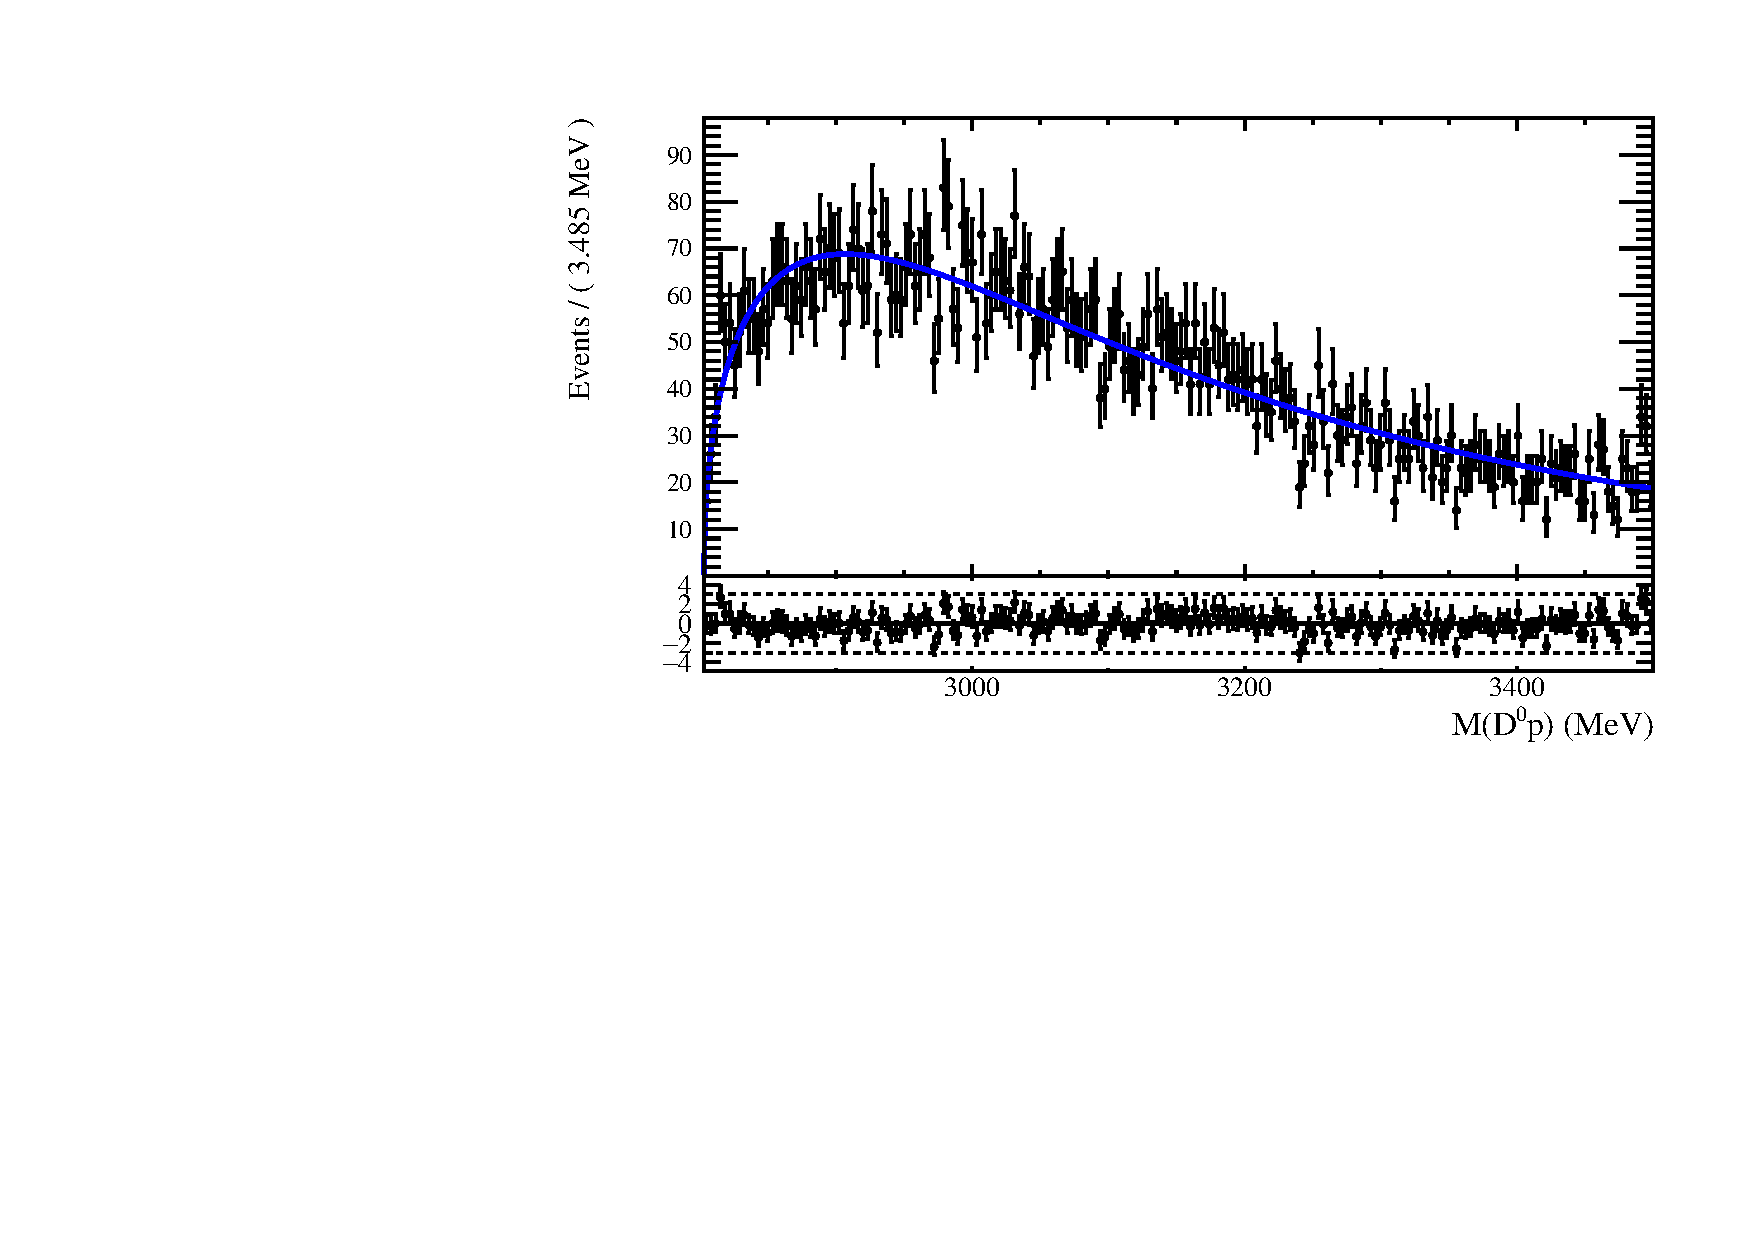
\includegraphics[width=0.49\textwidth]{LbToD0p/fits/data/mD0p_WSp/fit_EmpiricBG}
	\caption{Fit to \Dz\proton mass of WS proton events.}
    \label{fig:fit_mD0p_WS}
\end{figure}

Unfortunately, there isn't any reliable simulation predicting the mass shape for the \Dz\proton invariant mass. 
A shape for the signal therfore has to be determined empirically. The \Dz\proton mass is fitted with the requirement that the \Dz\proton\muon system makes a good vertex, i.e. $\logIP < 1$. 
This is a very signal rich region and should give a proper idea of the mass shape. 
The main part of the signal will be nonresonant but furthermore it is expected to see at least two resonances, namely the decays \decay{\LcResI}{\Dz\proton} and \decay{\LcResII}{\Dz\proton}.
These two resonances are parametrized by a relativistic Breit-Wigner distribution convoluted with a Gaussian $\mathcal{G}(m|m_0,\sigma)$ to account for the detector's massresolution.
\begin{align}
    \text{RelBW}(m|m_0,\Gamma) = \left[ 2m \cdot \text{PS}(m|m_1,m_2) \cdot \frac{1}{(m^2 -m_0^2)^2 + m_0^2\Gamma^2} \right] \otimes \mathcal{G}(m|m_0,\sigma), \label{eq:RelBW}
\end{align}
 Here $PS$ denotes the phase space function of eq (\ref{eq:PS}), $m_0$ the resonance's mass and $\Gamma$ its width.
 The determination of the mass resolution is described in section \ref{sec:Massresolution}. 
 The obtained resolution is then fixed in all fits.

The nonresonant signal part is modeled with the sum of two exponentials multiplied by a turnon function.
\begin{align}
    \text{TDExp}(m|m_0, c_0, c_1, c_2, f_{c_1}) = \left( 1 - \mathrm{e}^{c_0(m-m_0)} \right) \cdot \left[ f_{c_1} \mathrm{e}^{c_1m} + (1-f_{c_1}) \mathrm{e}^{c_2m} \right] \label{eq:TDExp}
\end{align}
This choice of turnon guarantees the function to rise as steep as necessary at \Dz\proton mass threshold.

When fitting the \Dz\proton mass it turns out, that this parametrization is not sufficient to describe the whole mass spectrum (see figure \ref{fig:fit_mD0p_RS} left). 
There is an enhancement at low \Dz\proton masses right after threshold.
Different models for the nonresonant component have been tried to describe this steep curvature without success.
A possible solution seems to be adding another component parametrized like the two resonances in the fit (fig. \ref{fig:fit_mD0p_RS} right). 
With this choice the fit converges and describes the data well.
The total fit function consists now of 4 parts: The nonresonant part modeled with the ``turnon double exponential" function TDExp of eq. (\ref{eq:TDExp}), the \LcResI, \LcResII and a low mass enhancement, each modeled with a relativistic Breit-Wigner according eq. (\ref{eq:RelBW}). 
The fitresults can be seen in figure \ref{fig:fit_mD0p_RS} (right) and table \ref{tab:fit_TurnOnDExp_3RelBWPSRes}.

Note that at this point, there is no special motivation to introduce this component (and model it like the resonances) except to get a converging and data matching fit.
There are several possible reasons for such an enhancement.
A thorough discussion, if this additional component is actually needed and what its origins could be can be found in section \ref{sec:Structure}.
In the following this component will be treated as signal since it appears very clear in the signal rich, i.e. low \logIP region and should does make a good decay vertex.
\begin{figure}[hptb]
    \centering
	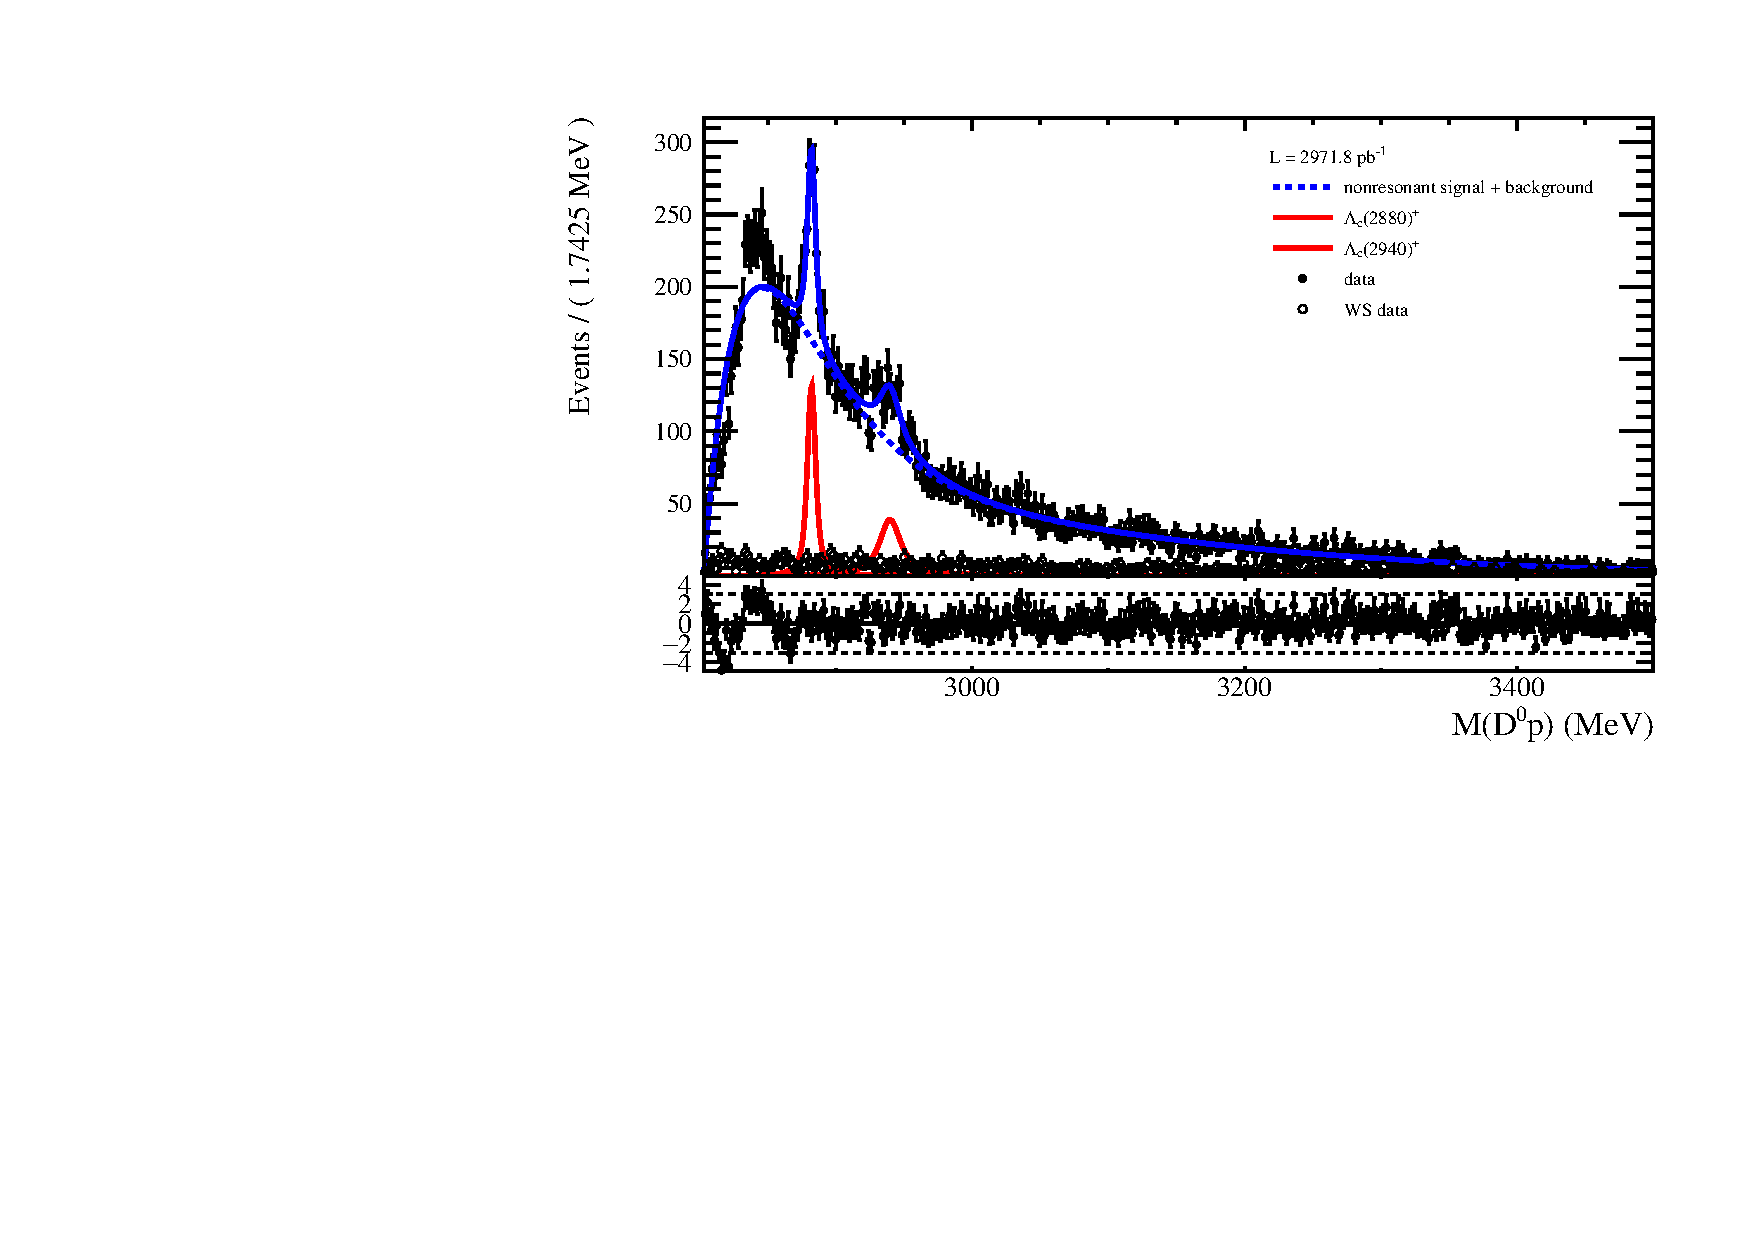
\includegraphics[width=0.49\textwidth]{LbToD0p/fits/data/mD0p_RS/fit_TurnOnDExp_2RelBWPSRes}
	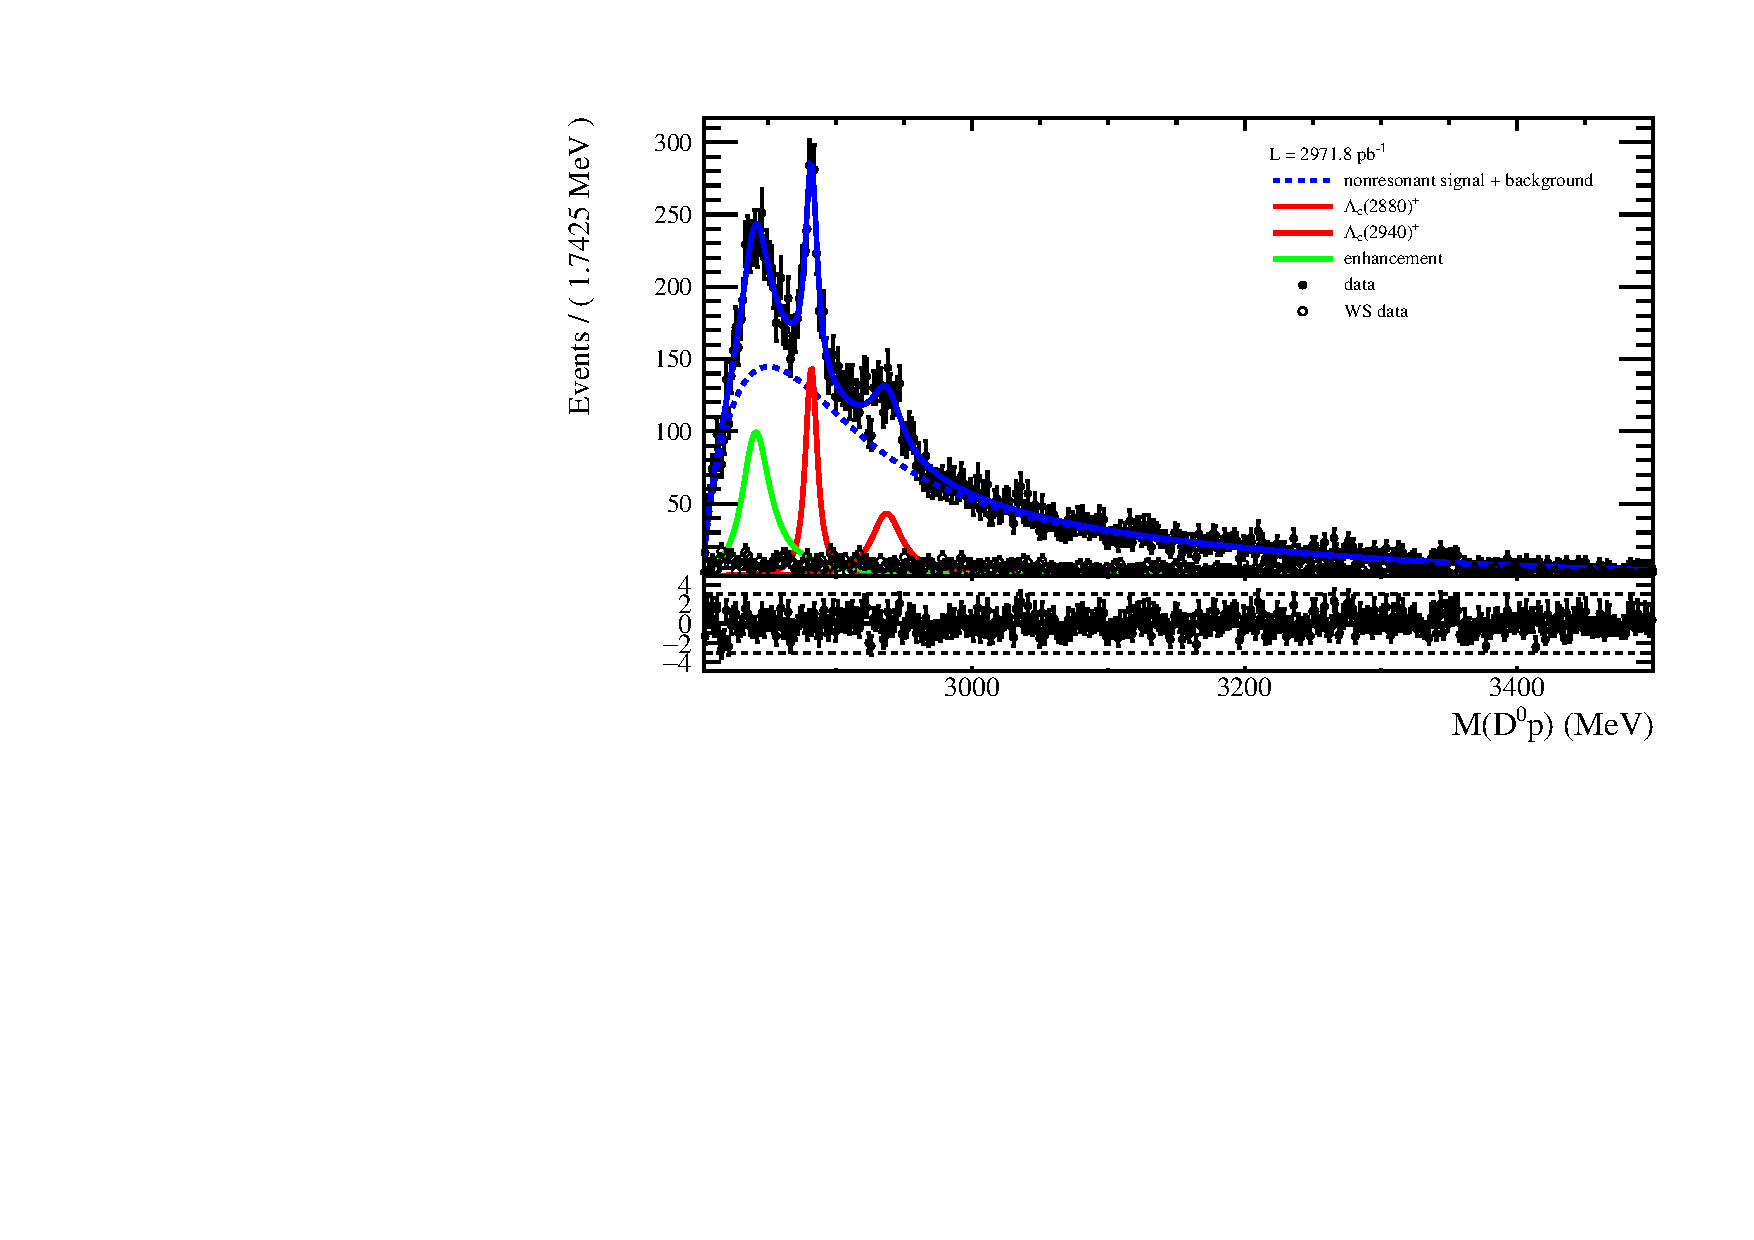
\includegraphics[width=0.49\textwidth]{LbToD0p/fits/data/mD0p_RS/fit_TurnOnDExp_3RelBWPSRes}
	\caption{1D fit of the \Dz\proton mass distribution for $\logIP < 1$. The left side shows a fit with two resonances and a nonresonant part. Different attempts have been made to get a proper and converging fit. This issue can be solved by adding an additional component (right figure, green line), here parametrized like the two resonances.}
    \label{fig:fit_mD0p_RS}
\end{figure}
 
\begin{table}[h]
    \centering
    \caption{Results of the \Dz\proton mass fit.}
    \label{tab:fit_mD0p_RS}
    $\begin{array}{lr@{\pm}l}
    \hline
    \text{Variable} & \multicolumn{2}{c}{\text{Value}} \\
    \hline
        \multicolumn{3}{l}{\text{\textbf{Yields}}} \\
\text{\LcResI signal yield}&(1.26 & 0.16) \cdot 10^{3}\\
\text{\LcResII signal yield}&(1.01 & 0.32) \cdot 10^{3}\\
\text{mass enhancement yield}&(2.12 & 0.44) \cdot 10^{3}\\
\text{nonresonant yield}&(1.65 & 0.08) \cdot 10^{4}\\
\multicolumn{3}{l}{\text{\textbf{\LcResI resonance}}} \\
\text{mean}&(2.88 & 0.00) \cdot 10^{3}\\
\text{width}&(8.90 & 1.40) \cdot 10^{0}\\
\multicolumn{3}{l}{\text{\textbf{\LcResII resonance}}} \\
\text{mean}&(2.94 & 0.00) \cdot 10^{3}\\
\text{width}&(2.62 & 0.79) \cdot 10^{1}\\
\multicolumn{3}{l}{\text{\textbf{Low mass enhancement}}} \\
\text{mean}&(2.84 & 0.00) \cdot 10^{3}\\
\text{width}&(2.44 & 0.37) \cdot 10^{1}\\
\multicolumn{3}{l}{\text{\textbf{nonresonant part}}} \\
\text{turn on mass threshold}&(2.80 & 0.00) \cdot 10^{3}\\
\text{turn on slope}&(-2.00 & 32.00) \cdot 10^{-5}\\
\text{exponential 1 slope}&(-2.34 & 0.13) \cdot 10^{-2}\\
\text{exponential 2 slope}&(-7.07 & 0.20) \cdot 10^{-3}\\
\text{fraction exponential 1}&(7.40 & 0.24) \cdot 10^{-1}\\

\hline
\end{array}$
\end{table}
    

\section{Determination of the massresolution}
\label{sec:Massresolution}
If one sees a resonance in a mass spectrum, it isn't usually the natural width of a resonance which is seen.
The reason lies in the fact that the detector has a finite massresolution ``overlapping" the natural width.
In this analysis the effect is accounted for by convoluting the Breit-Wigner, which is assumed to be the natural shape of the resonance, with a Gaussian, describing the smearing of the resonance due to massresolution.

The determination of the massresolution makes use of a simulation.
For that purpose, the \Dz\proton mass spectrum is split up in bins of 30\mev.
For each mass bin a histogram is filled with the difference of the generated (also called ``true") and the reconstruted mass in the simulation.
It is expected that this difference peaks around zero.
Finally, a fit is performed on these histograms using a simple Gaussian function.
The width of this Gaussian is then assumed to be the massresolution in the particular bin.
Figure \ref{fig:massresolution} shows on the left side exemplarily the massdifference between reconstructed and generated mass together with the fit in the bin $2863 < M(\Dz\proton) < 2893 \mev$. 
The fits of all bins can be seen in Appendix \ref{app:Massresolution}, figure \ref{fig:massresolution_all}.
On the right side, the obtained massresolutions for all bins are plotted.
The higher the bin, the larger the errors are due to less statistics in these bins.
Since only the bins containing the resonances are of particular interest, these larger errors doesn't matter for this study.
\begin{figure}[hptb]
    \centering
	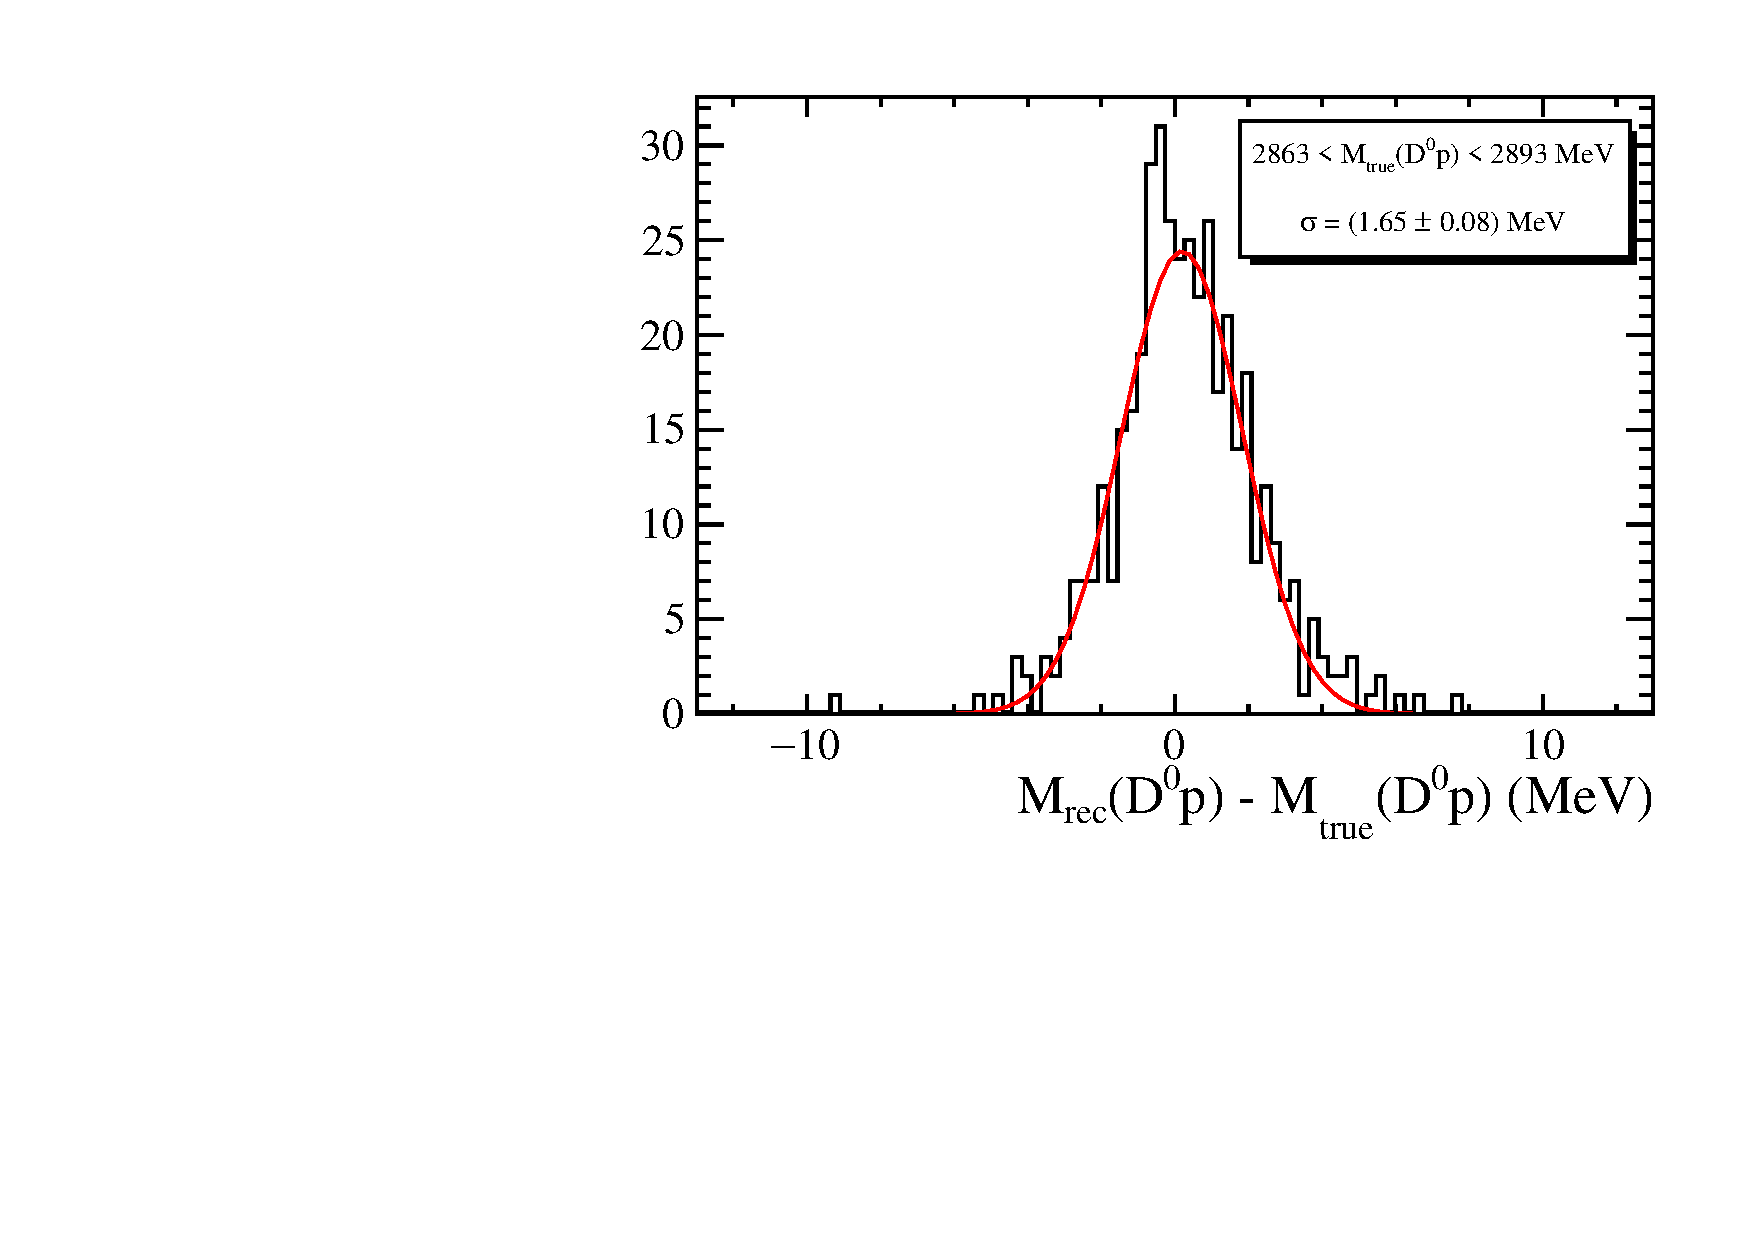
\includegraphics[width=0.49\textwidth]{LbToD0p/massresolution/massresolution_002}
	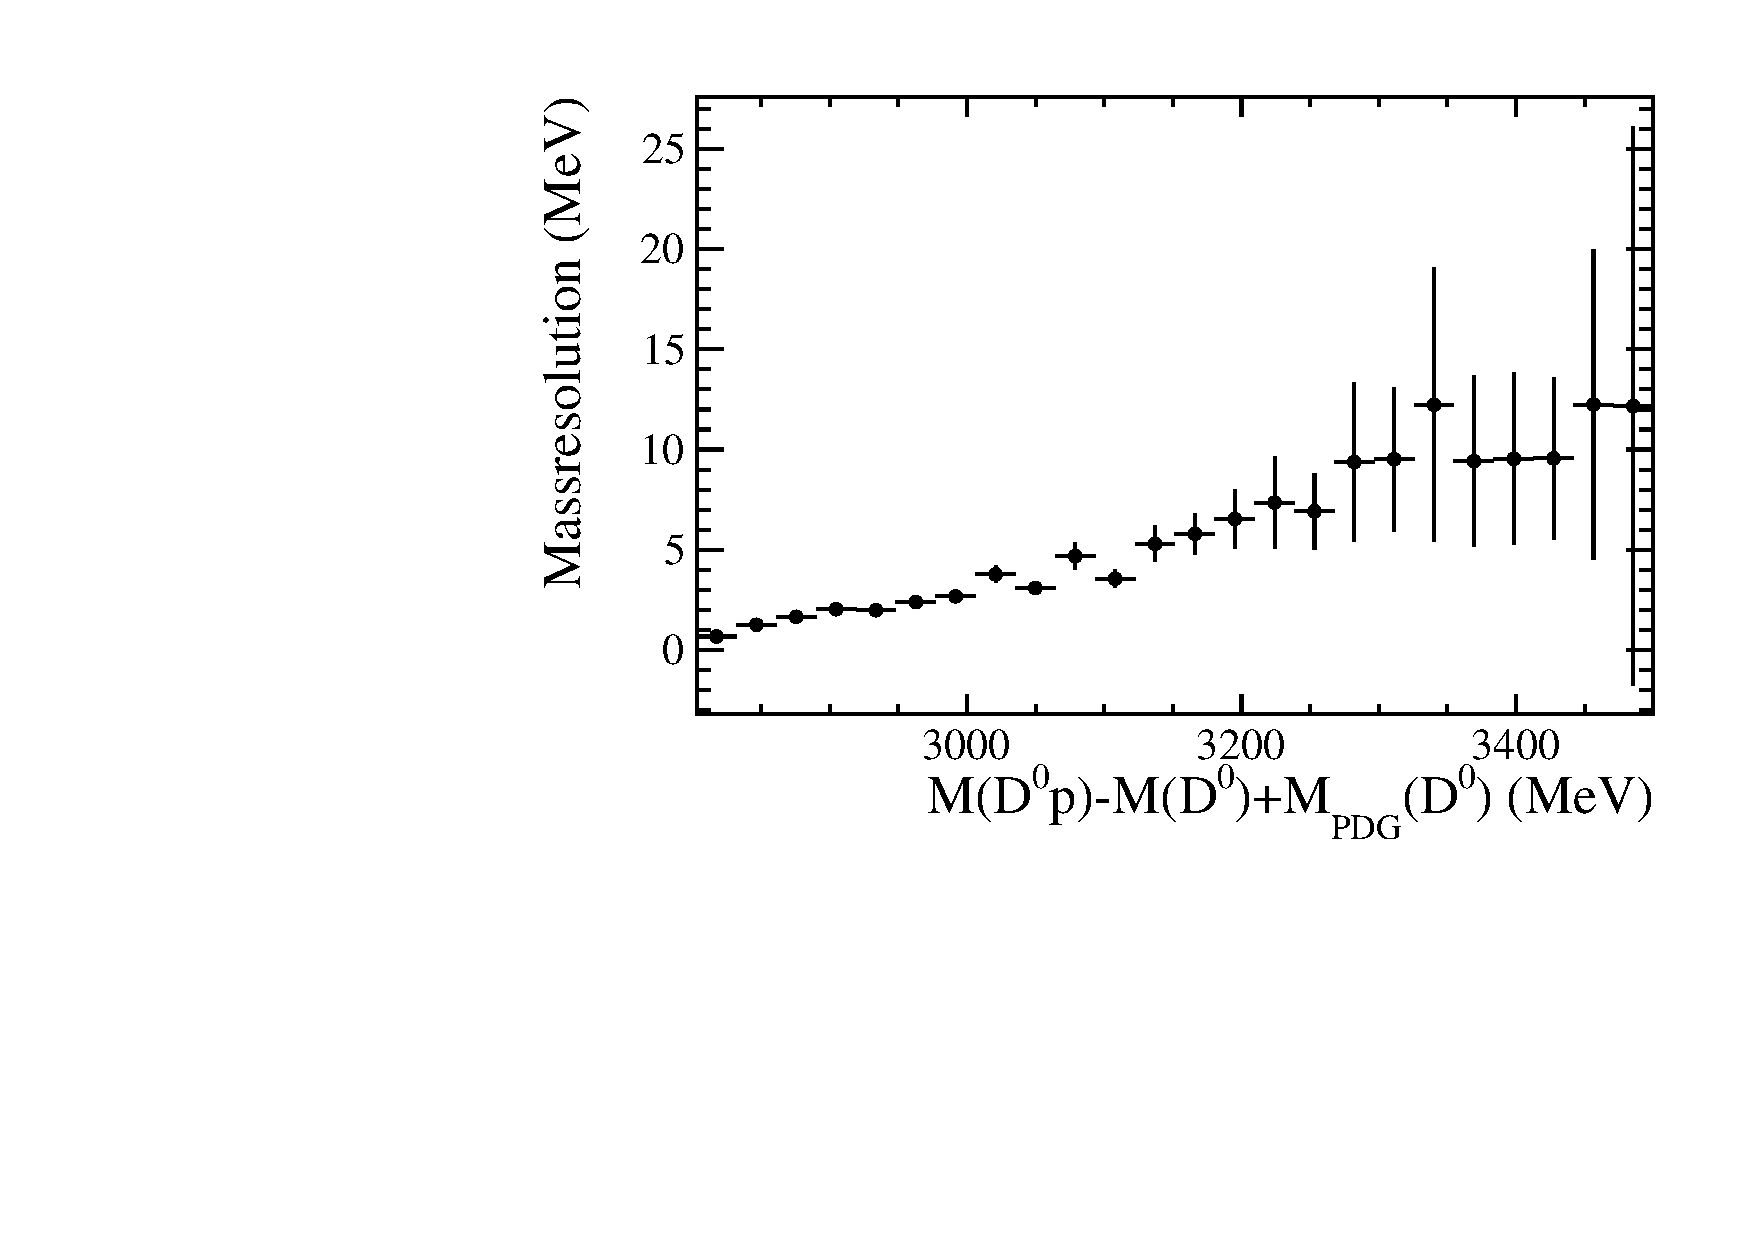
\includegraphics[width=0.49\textwidth]{LbToD0p/massresolution/massresolution_widths}
	\caption{Left: Fit of a Gaussian to the difference between generated and reconstructed \Dz\proton mass (simulation sample) in the range $2863 < M(\Dz\proton) < 2893 \mev$. The width of the Gaussian is taken as massresolution. Right: Obtained massresolutions for all bins. 
             The large errors in the higher bins doesn't matter for the desired purpose as only the bins containing the resonances are relevant.}
    \label{fig:massresolution}
\end{figure}

Regarding these results, the \LcResI, \LcResII and the enhancement are fitted with the following fixed massresolutions:
\begin{align*}
    \LcResI:           && \sigma_{M,\LcResI}            &= (\MassresResIval \pm \MassresResIerr) \mev, \\
    \LcResII:          && \sigma_{M,\LcResII}           &= (\MassresResIIval \pm \MassresResIIerr) \mev, \\
    \text{enhancement}:&& \sigma_{M,\text{enhancement}} &= (\MassresStructureval \pm \MassresStructureerr) \mev.
\end{align*}

\section{Nominal fit in two dimensions}
\label{sec:Fit_2D}
With a twodimensional fit of the \Dz\proton mass and the \logIP distribution it is possible to distinguish between nonresonant signal and background in the \Dz\proton mass spectrumi as already explained.
Thus the different pieces of the previous sections are now put together for a fit of both distributions.

It is assumed that the \logIP distribution is the same for all 4 different signal components (nonresonant signal, \LcResI, \LcResII, enhancement).
This assumption bases on the fact that the decay topology should be the same in all cases\footnote{Presumed, that the enhancement indeed emerges to be a resonance or another signal component.}.
Hence, their \logIP distributions share all parameters. For the \logIP signal part a double Bifurcated Gaussian \DBfG is chosen, whereas the background is modeled by a CrystalBall function \CB.
The \Dz\proton mass' signal components are modeled with the same parametrization as described in section \ref{sec:mD0p_signal_shape}. 
The empiric background function EBG is used to describe the background.

Table \ref{tab:fit_2D_model} summarizes the parametrization of the entire twodimensional fit. The results of the fit are shown in table \ref{tab:2Dfit} and the projections can be seen in figure \ref{fig:fit2D}.

\begin{table}[hptb]
    \centering
    \caption{Summary of the parameterization of the 2D fit}
    \label{tab:fit_2D_model}
    \begin{tabular}{l||l|l}
        subset              & mass distribution            & logIP distribution                            \\ \hline \hline
        non-resonant signal & TDExp (eq. \ref{eq:TDExp})   & \multirow{4}{*}{Double Bifurcated Gaussian}   \\ \cline{1-2}
        \LcResI resonance   & RelBW (eq. \ref{eq:RelBW})   &                                               \\ \cline{1-2}
        \LcResII resonance  & RelBW (eq. \ref{eq:RelBW})   &                                               \\ \cline{1-2}
        enhancement         & RelBW (eq. \ref{eq:RelBW})   &                                               \\ \hline
        background          & EBG (eq. \ref{eq:EBG}        & CrystalBall
    \end{tabular}
\end{table}

\begin{figure}[hptb]
	\centering
	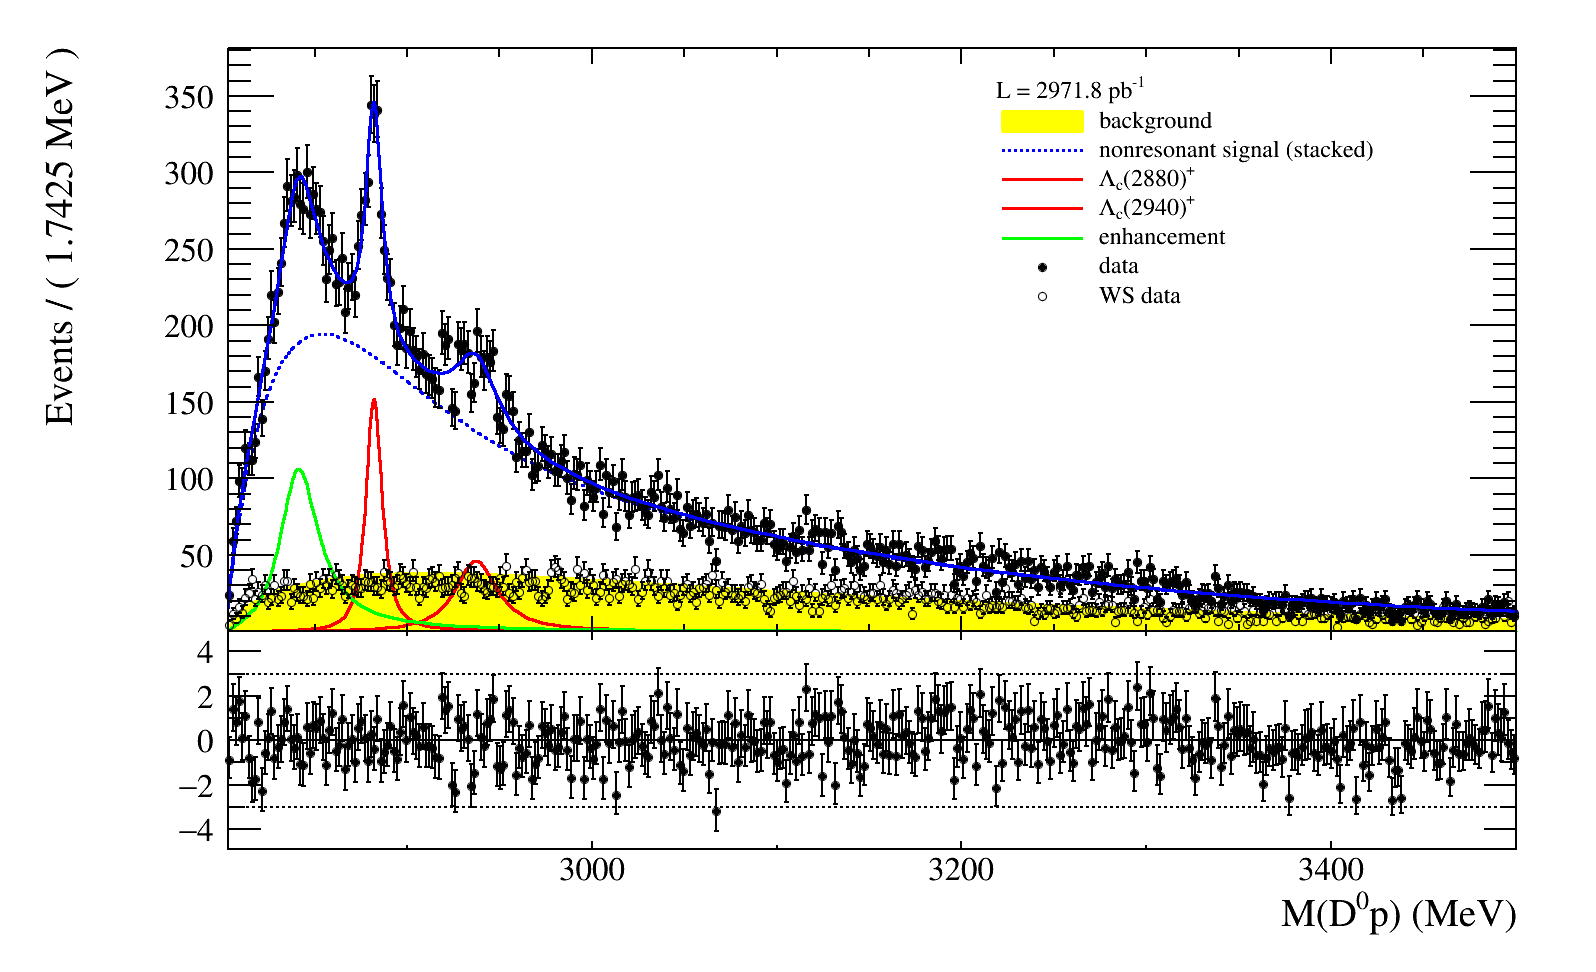
\includegraphics[width=\textwidth]{LbToD0p/fits/data/2Dfit/fit_DBfG_CB_vs_TurnOnDExp_3RelBWPSRes_EmpiricBG_mD0pProj} \\
	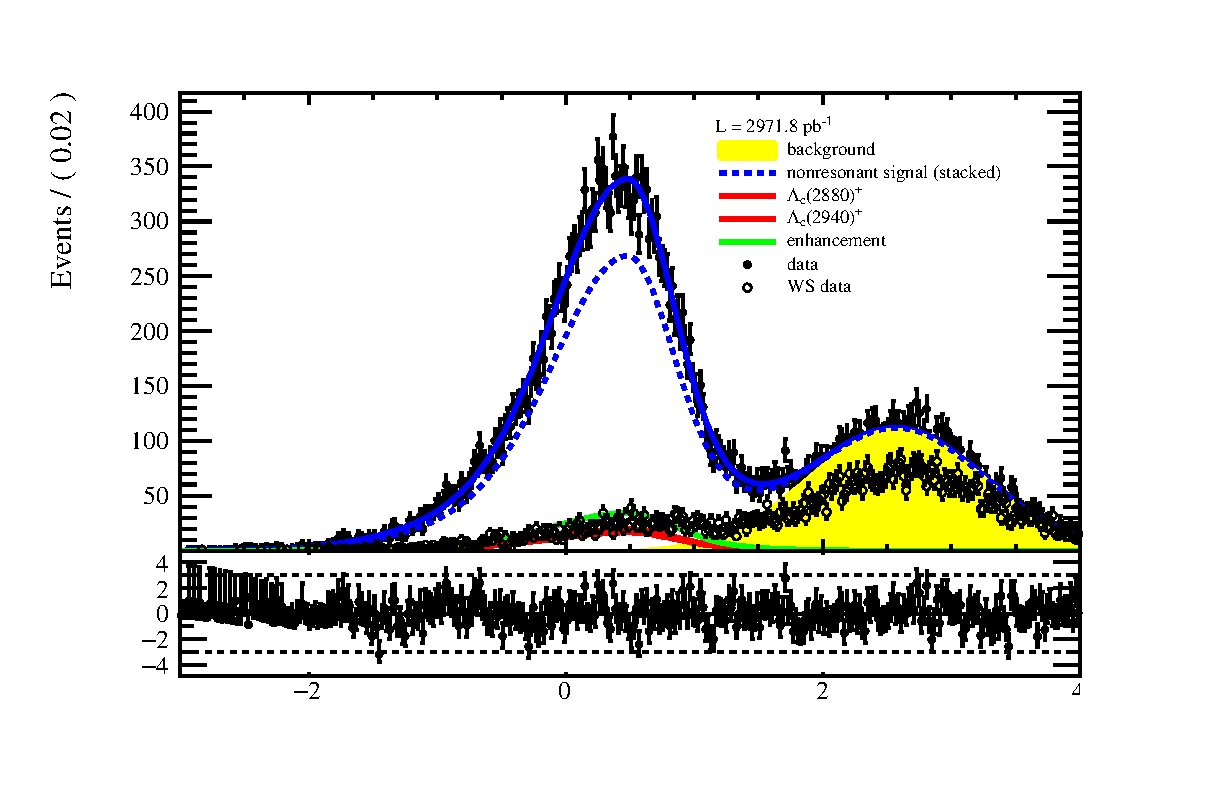
\includegraphics[width=\textwidth]{LbToD0p/fits/data/2Dfit/fit_DBfG_CB_vs_TurnOnDExp_3RelBWPSRes_EmpiricBG_logIPProj}
	\caption{Twodimensional fit on the \LbToDpmunuX candidates. There are shown the \Dz\proton mass (top) and \logIP (bottom) projection. The total fit parametrization is summarized in table \ref{tab:fit_2D_model}.}
	\label{fig:fit2D}
\end{figure}
 
\begin{table}[h]
    \centering
    \caption{Results of the twodimensional M(\Dz\proton) and \logIP fit.}
    \label{tab:2Dfit}
    $\begin{array}{lr@{\pm}l}
    \hline
    \text{Variable} & \multicolumn{2}{c}{\text{Value}} \\
    \hline
        \multicolumn{3}{l}{\text{\textbf{Yields}}} \\
\text{\LcResI signal yield}&(1.28 & 0.15) \cdot 10^{3}\\
\text{\LcResII signal yield}&(1.06 & 0.24) \cdot 10^{3}\\
\text{mass enhancement yield}&(2.29 & 0.45) \cdot 10^{3}\\
\text{nonresonant signal yield}&(1.83 & 0.069) \cdot 10^{4}\\
\text{background yield}&(9.42 & 0.14) \cdot 10^{3}\\
\multicolumn{3}{l}{\text{\textbf{\LcResI resonance}}} \\
\text{mean [\mev]}&(2.88197 & 0.00034) \cdot 10^{3}\\
\text{width [\mev]}&(7.4 & 1.3) \cdot 10^{0}\\
\multicolumn{3}{l}{\text{\textbf{\LcResII resonance}}} \\
\text{mean [\mev]}&(2.9374 & 0.0016) \cdot 10^{3}\\
\text{width [\mev]}&(2.44 & 0.55) \cdot 10^{1}\\
\multicolumn{3}{l}{\text{\textbf{Low mass enhancement}}} \\
\text{mean [\mev]}&(2.84222 & 0.00088) \cdot 10^{3}\\
\text{width [\mev]}&(2.51 & 0.37) \cdot 10^{1}\\
\multicolumn{3}{l}{\text{\textbf{Nonresonant signal}}} \\
\text{turn on mass threshold [\mev]}&(2.80127 & 0.00057) \cdot 10^{3}\\
\text{turn on slope [\mev$^{-1}$]}&(-2.0 & 36.0) \cdot 10^{-4}\\
\text{exponential 1 slope [\mev$^{-1}$]}&(-2.34 & 0.14) \cdot 10^{-2}\\
\text{exponential 2 slope [\mev$^{-1}$]}&(-7.03 & 0.78) \cdot 10^{-3}\\
\text{fraction exponential 1}&(7.36 & 0.25) \cdot 10^{-1}\\
\multicolumn{3}{l}{\text{\textbf{Background (mass)}}} \\
\text{Empiric BG $c_1$ [\mev$^{-1}$]}&(-1.595 & 0.05) \cdot 10^{1}\\
\text{Empiric BG $p_0$}&(5.6 & 3.0) \cdot 10^{-2}\\
\multicolumn{3}{l}{\text{\textbf{Signal (\logIP)}}} \\
\text{mean}&(4.8 & 0.16) \cdot 10^{-1}\\
\text{left width 1}&(9.76 & 0.27) \cdot 10^{-1}\\
\text{right width 1}&(6.22 & 0.32) \cdot 10^{-1}\\
\text{left width 2}&(5.37 & 0.24) \cdot 10^{-1}\\
\text{right width 2}&(3.41 & 0.15) \cdot 10^{-1}\\
\text{fraction BfG 1}&(4.21 & 0.42) \cdot 10^{-1}\\
\multicolumn{3}{l}{\text{\textbf{Background (\logIP)}}} \\
\text{CB mean}&(2.573 & 0.012) \cdot 10^{0}\\
\text{CB $\sigma$}&(6.87 & 0.11) \cdot 10^{-1}\\
\text{CB $\alpha$}&(7.1 & 3.8) \cdot 10^{0}\\
\text{CB $n$}&(3.0 & 1.4) \cdot 10^{0}\\

\hline
\end{array}$
\end{table}
    

% ==================================
% Subsection: Control of the method
% ==================================
\section{Control of the method and parametrization}

As a control the two dimensionsal fit is performed for the WS data with the same parametrization as for the RS in section \ref{sec:Fit_2D}.
However, since there shouldn't be any resonances, these two components and the enhancement have been omitted.
The respective plots can be seen in figure \ref{fig:fit_2D_WS}. 
No structure in the mass distribution is seen. 
This means that the identification of the \LcResI and \LcResII in the \Dz\proton mass spectrum seems to be appropriate.
Interesting is to note, that besides th two resonances even the enhancement vanishes.
It can't thus be explained by random combinations of the particles.
Concerning the \logIP distribution, there is nevertheless a ``signal-like" part which has to be discussed in the backgrounds chapter \ref{sec:Backgrounds}.

\begin{figure}[hptb]
	\centering
	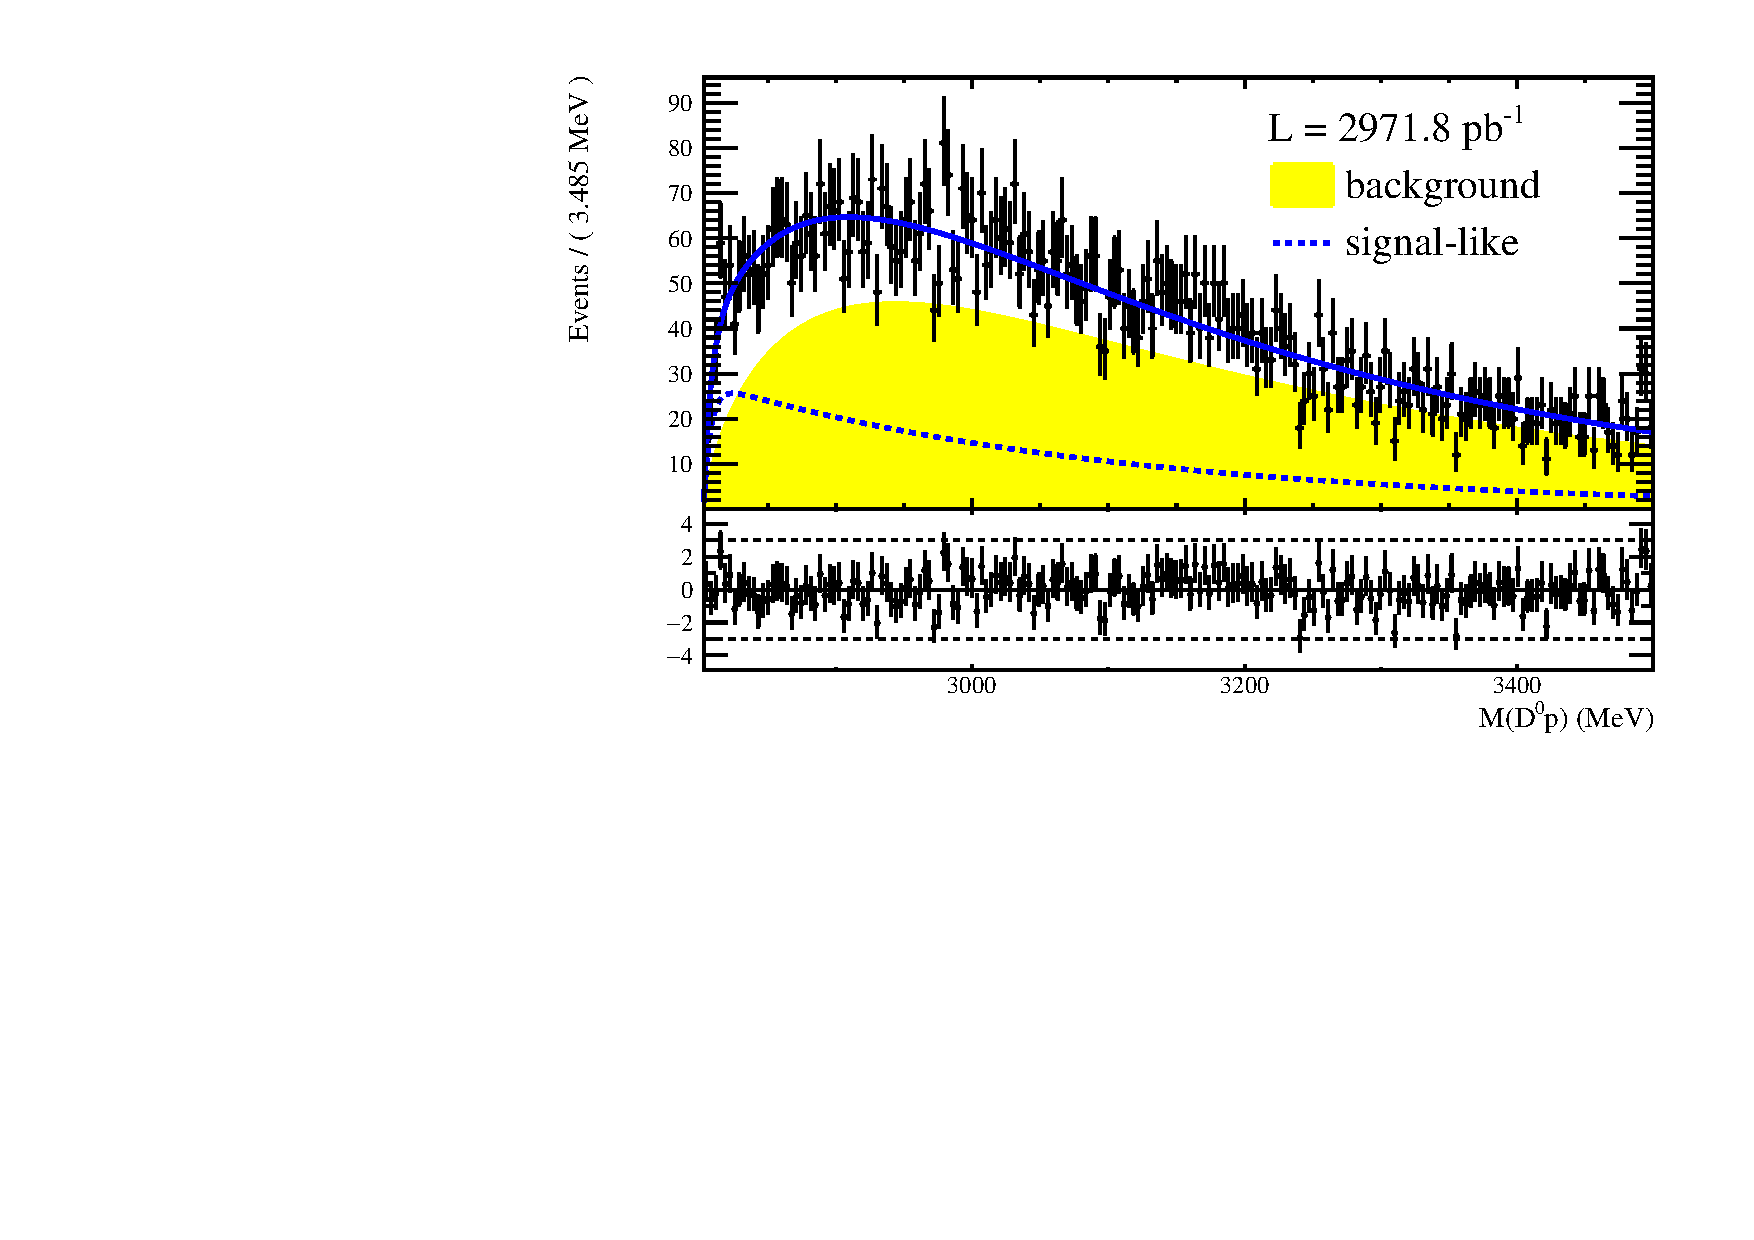
\includegraphics[width=0.49\textwidth]{LbToD0p/fits/data/2DWSfit/fit_DBfG_CB_vs_TurnOnDExp_EmpiricBG_mD0pProj}
	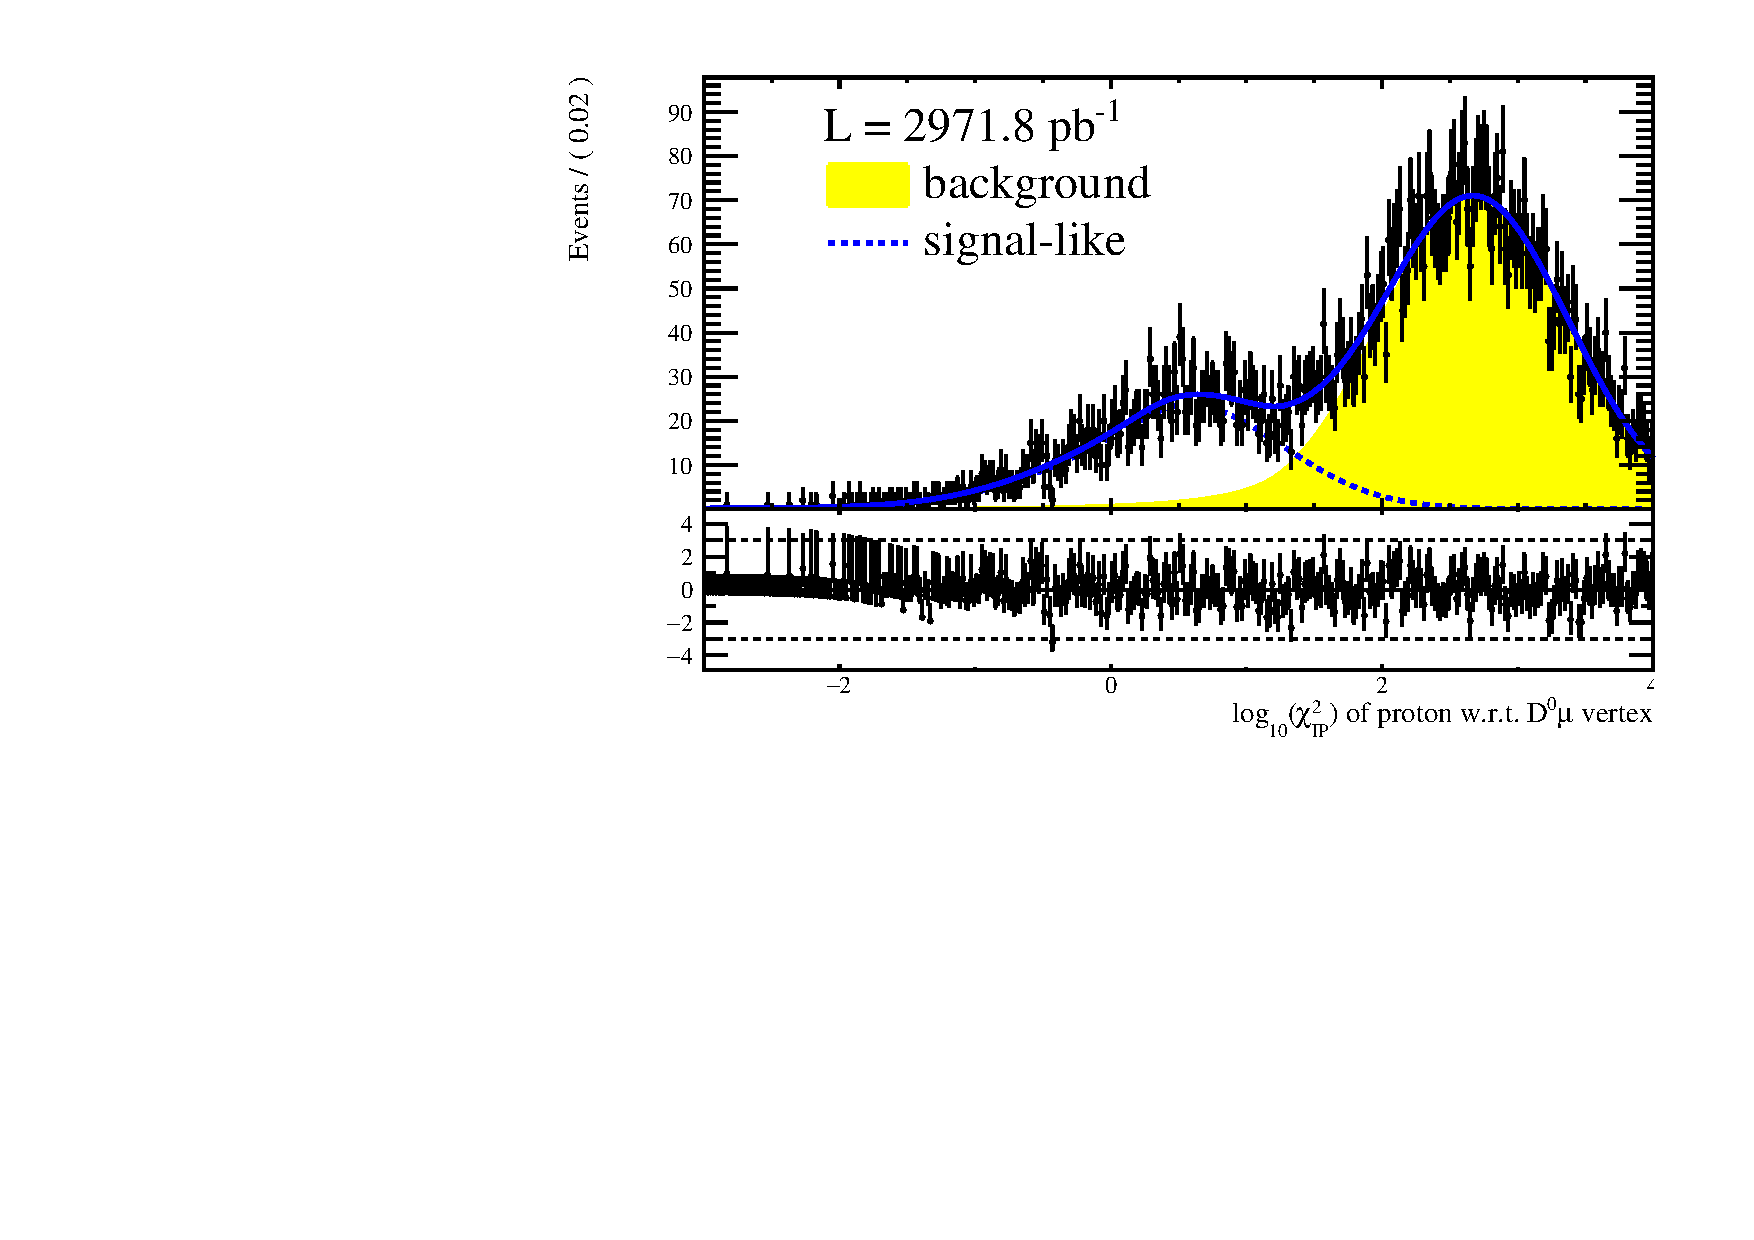
\includegraphics[width=0.49\textwidth]{LbToD0p/fits/data/2DWSfit/fit_DBfG_CB_vs_TurnOnDExp_EmpiricBG_logIPProj}
	\caption{Invariant mass (left) and \logIP (right) distribution for ``wrong sign" (WS) candidates.}
	\label{fig:fit_WS}
\end{figure}


% ==================================
% Subsection: Signal yield and resonances
% ==================================
\section{Extraction of \LbToDpmunuX signal yield together with \LcResI and \LcResII properties}

From the previous fits different results can be obtained. 
Concerning the 2Dfit (see tab. \ref{tab:2Dfit} the yields for the components nonresonant signal, \LcResI, \LcResII and enhancement are summed up to get the total \LbToDpmunuX signal yield \NDp for the calculation of \R. The number is
\begin{align*}
    \NDp = (\NDpvalscient \pm \NDperrscient)\cdot 10^{\NDpexpscient}. 
\end{align*}

From the \Dz\proton mass spectrum it is furthermore possible to measure the masses and widths of the \LcResI and \LcResII resonances. In this case it isn't needed to distinguish between nonresonant signal and background. 
To avoid uncertainties caused by this distinction, the onedimensional fit of the \Dz\proton mass (see tab. \ref{tab:fit_mD0p_RS} is used to get the properties of the two resonances:
\begin{align*}
    \LcResI: \qquad  m_{\LcResI}       &= (\LcResImeanval \pm \LcResImeanerr) \mev, \\
                     \Gamma_{\LcResI}  &= (\LcResIwidthval \pm \LcResIwidtherr) \mev, \\
    \LcResII: \qquad m_{\LcResII}      &= (\LcResIImeanval \pm \LcResIImeanerr) \mev, \\
                     \Gamma_{\LcResII} &= (\LcResIIwidthval \pm \LcResIIwidtherr) \mev. \\
\end{align*}
